%%%%%%%%%%%%%%%%%%%%%%%%%%
% MSc Project Background Report Template
% Prof. Roger K. Moore
% University of Sheffield
% 22 March 2017
%%%%%%%%%%%%%%%%%%%%%%%%%%


\documentclass[11pt,oneside]{book}
\usepackage[margin=1.2in]{geometry}
\usepackage{setspace}
\usepackage[toc,page]{appendix}
\usepackage[none]{hyphenat} % turn hyphenation off by default
\usepackage{graphicx}

\newcommand{\mycomment}[1]{}

\begin{document}

\frontmatter

\begin{titlepage}

% You need to edit the details here

\begin{center}
{\LARGE University of Sheffield}\\[1.5cm]
\linespread{1.2}\huge {\bfseries Understanding Elderly Speech Recognition}\\[1.5cm]
\linespread{1}

\includegraphics[width=5cm]{images/tuoslogo}\\[1cm]
{\Large Adam Spencer}\\[1cm]
{\large \emph{Supervisor:} Professor Jon Barker}\\[1cm]
\large A report submitted in partial fulfilment of the requirements\\ for the degree of B.Sc. in
Artificial Intelligence and Computer Science\\ (COM3610)\\[0.3cm]
\textit{in the}\\[0.3cm]
Department of Computer Science\\[2cm]
\today
\end{center}

\end{titlepage}

% -------------------------------------------------------------------
% Declaration
% -------------------------------------------------------------------

\newpage
\chapter*{\Large Declaration}

\setstretch{1.1} % set the line spacing differently if you wish, but this looks good to me. 

All sentences or passages quoted in this report from other people's work have been specifically
acknowledged by clear cross-referencing to author, work and page(s).
Any illustrations that are not the work of the author of this report have been used with the
explicit permission of the originator and are specifically acknowledged.
I understand that failure to do this amounts to plagiarism and will be considered grounds for
failure in this project and the degree examination as a whole.\\[1cm]

\noindent Name: \quad Adam Spencer\\[1mm]
\rule[1em]{25em}{0.5pt}

\noindent Signature:\\[1mm]
\rule[1em]{25em}{0.5pt}

\noindent Date: \quad \today\\[1mm]
\rule[1em]{25em}{0.5pt}

% -------------------------------------------------------------------
% Abstract
% -------------------------------------------------------------------

\chapter*{\Large \center Abstract}

Lorem ipsum dolor sit amet, consectetuer adipiscing elit. Aenean commodo ligula eget dolor. Aenean massa. Cum sociis natoque penatibus et magnis dis parturient montes, nascetur ridiculus mus. Donec quam felis, ultricies nec, pellentesque eu, pretium quis, sem. Nulla consequat massa quis enim. Donec pede justo, fringilla vel, aliquet nec, vulputate eget, arcu. In enim justo, rhoncus ut, imperdiet a, venenatis vitae, justo. Nullam dictum felis eu pede mollis pretium. Integer tincidunt. Cras dapibus. Vivamus elementum semper nisi. Aenean vulputate eleifend tellus. Aenean leo ligula, porttitor eu, consequat vitae, eleifend ac, enim. Aliquam lorem ante, dapibus in, viverra quis, feugiat a, tellus. Phasellus viverra nulla ut metus varius laoreet. Quisque rutrum. Aenean imperdiet. Etiam ultricies nisi vel augue. Curabitur ullamcorper ultricies nisi. Nam eget dui. Etiam rhoncus. Maecenas tempus, tellus eget condimentum rhoncus, sem quam semper libero, sit amet adipiscing sem neque sed ipsum. Nam quam nunc, blandit vel, luctus pulvinar, hendrerit id, lorem. Maecenas nec odio et ante tincidunt tempus. Donec vitae sapien ut libero venenatis faucibus. Nullam quis ante. Etiam sit amet orci eget eros faucibus tincidunt. Duis leo. Sed fringilla mauris sit amet nibh. Donec sodales sagittis magna. Sed consequat, leo eget bibendum sodales, augue velit cursus nunc.


% -------------------------------------------------------------------
% TOC etc
% -------------------------------------------------------------------

\tableofcontents
\listoffigures
\listoftables

\setstretch{1.1} 

\mainmatter

\chapter{Introduction}\label{ch:introduction}

Automatic Speech Recognition systems are rapidly increasing in accuracy, from 17.1\% word error
rate (WER) in 2011~\cite{seide2011} to 5.1\% in 2021~\cite{Ng2021} on the same Switchboard
corpus~\cite{switchboard}.
Though this increase in accuracy is promising for the average English speaker, elderly speakers
have different speech patterns~\cite{Horton2010} and are transcribed less accurately than other age
groups~\cite{picone1990}.

\\
The objective of this work is to provide an in-depth understanding of how the differences
between elderly and non-elderly speech influence the accuracy of different types of ASR systems,
and which (if any) current models best fit the task of transcribing elderly speech.

\section{Overview of the Report}\label{sec:overview-of-the-report}


\chapter{Literature Survey}\label{ch:literature-survey}

\section{Modern ASR}\label{sec:modern-asr}

The results of ASR models are reported as a percentage word error rate (WER), meaning the
percentage of words produced by the model which are incorrect compared to the real transcript (i
.e. lower WER means higher accuracy).\\

In late September 2022, the OpenAI research laboratory (known for their `GPT-3' language model)
released a new open-source ASR system known as `Whisper'~\cite{whisper}.
Whisper is unique in being very large (trained on 680,000 hours of speech data), open-source, and
fully supervised;
meaning all the training data used to create the model has been accurately labeled and
quality-checked by humans, unlike the much larger unsupervised `BigSSL' model (1,000,000+ hours
of data)~\cite{bigssl}.

Their accuracy results are promising across a range of different speech corpora, outperforming
previous state-of-the-art \emph{wav2vec 2.0}~\cite{wav2vec}.
Interestingly, Whisper doesn't achieve higher performance than some other models on specific
corpora, for example on \emph{LibriSpeech test-other}~\cite{librispeech} it is outperformed by
two models built atop \emph{wav2vec}~\cite{zhang2020,chung2021}, though across a more diverse set
of speech corpora Whisper achieves much higher lower WER~\cite{whisper}.\\

\section{Elderly Speech}\label{sec:elderly-speech}



\section{Data Collection}\label{sec:data-collection}

The key requirement for comparing these systems is a large dataset of speech recordings over a
wide range of ages, with labels denoting the age of the speaker and an accurate transcript to
compare ASR performance against.
There is a surprising lack of relevant resources online, with most speech corpora featuring
labeled speaker age not featuring a diverse age range.

The LifeLUCID Corpus is, however, collected with the express purpose of providing a wide range of
speaker ages~\cite{lifelucid}.
This resource has great potential in providing an insight into the age-variable performance of
ASR because it features 104 British English speakers between 8 and 85 years of age.

It is of interest to observe any patterns in errors made by each system, especially if there are
any similarities in where they lose accuracy.
Once the areas of error are understood, comparing and contrasting audio spectra may allow for
insight into which features of speech create problems for ASR .


\chapter{Requirements and Analysis}\label{ch:req-and-analysis}

The objective of this work is not to produce a fully-working, infallible system which aims to receive actual use by transcribers, rather, the aim of this work is to explore the current state of the field of ASR and to understand the extent that current ASR technology could provide aid to a human transcriber.
With the purpose of facilitating an extensive evaluation, this chapter shall list the requirements for this work to meet its objective and provide a detailed analysis of each requirement.

\section{Understand the motivations of computer-aided transcription}

\mycomment{
  TODO:
  * Rewrite / expand on this
  * define a 'target user'
  * actually motivate semi auto transcription!
}
Before exploring how a computer system may aid a human transcriber, it is important to understand;

\begin{itemize}
        \item \emph{why} a human transcriber may require aid;
        \item to \emph{whom} a computer-aided transcription system would provide benefit; and
        \item what the \emph{extent} of such a benefit would be.
\end{itemize}

If this report does not properly motivate computer-aided transcription to a reader, it will have partially failed in its purpose 

\section{Generate transcripts using ASR}\label{sec:generate-transcripts}

Evaluating the quality of ASR transcription requires a key set of data; ASR-generated transcripts.
Rather than comparing different ASR systems, Whisper\cite{whisper} has been chosen as the only system to use for generating transcripts because;

\begin{itemize}
        \item it is new (made available in September 2022);
        \item it is entirely free and open-source, meaning it is easily modifiable and available to be used without licence; and
        \item it reportedly achieves very good results across different speech corpora.
\end{itemize}

As mentioned in the literature review, Whisper is implemented using \emph{PyTorch}, meaning this work would benefit greatly from access to high-performance GPUs.
This would enable fast turnaround times when transcribing large speech corpora and thus enable rapid evaluation and tweaking of settings to minimise erroneous results.

The key to generating useful transcripts is some high-quality speech recordings from a speech corpus.
While preliminary testing of Whisper may use data from any available corpora, it would be very useful to obtain some data which is;

\begin{itemize}
        \item not present in Whisper's training data, to prevent the model from regurgitating labels for data it has already seen;
        \item is well-suited to Whisper's particularities, aiming to maximise the usefulness of results; and
        \item is representative of real data which would benefit from computer-aided transcription, as to enable more practical evaluation.
\end{itemize}

Two preliminary aims, therefore, are to understand what kind of data is suited to Whisper and then what kind of data would benefit from computer-aided transcription.
Once these aims are understood, a suitable dataset may be gathered and used for evaluation, however it is also useful to understand the caveats related to using well-suited data!
The na\"{i}ve assumption that all data seen by \emph{any} computer system is 'perfect' would misrepresent the usefulness of the system in question.
To combat this, this work must properly acknowledge the limited extent to which a computer-aided transcription system using Whisper is viable, and evaluate how the viability could be increased to be more applicable to real-world tasks.

\section{Implement various confidence measures}

Neural network confidence is widely discussed in the literature.
Considering the aim of this work, it shall focus on re-creating and applying existing measures of confidence to Whisper, whether through modification to the model itself or through inference of the model's output.

If some such modifications fall out of scope of the project, this work would still benefit from a discussion of how those approaches may be applied to a future system and what advantages they may bring.

\section{Understand the effectiveness of selected confidence measures}

Evaluation of the extent to which Whisper may aid human transcription may be done by comparing the accuracy of Whisper's predictions against a reference and the reported model confidence.

This type of evaluation requires taking the following steps to complete;

\begin{enumerate}
        \item Selection of suitable measure(s) of system accuracy
        \item Extensive normalisation of text to facilitate accurate measurements
        \item Visualisation of results
\end{enumerate}

The standard across surveyed literature is \emph{word error rate} (WER), despite potential limitations.
For the sake of evaluation, other measurements such as \emph{phone error rate} (PER) and \emph{character error rate} (CER) should be calculated alongside WER.

\section{Explore designs for computer-aided transcription}

It would be of great utility to understand how system confidence may aid a human transcriber as this would further refine the 'lens' through which the system may be evaluated, and as such is vital to the completion of this work.
There's limited use in a purely theoretical exploration of a computer system such as this, which is designed to be interfaced with by a human.
Instead, demonstrating the benefits of a computer-aided transcription system would be easily facilitated using a graphical program.

A number of considerations are required for the design of this system specifically due to its intended nature to serve as an example rather than a final implementation, including;

\begin{itemize}
        \item several design iterations should be produced to demonstrate different extents of computer aid;
        \item each design decision should be discussed thoroughly to demonstrate the intended effect and any notable caveats; and
        \item a suitable number of screenshots are required in the appendix to demonstrate use of the system.
\end{itemize}

\section{Evaluation}

\section{Ethical, Professional and Legal Issues}


\chapter{Design}\label{ch:design}

\section{Speech Data}

According to its authors, Whisper's robustness is due likely in part to its use of a language model in its decoder\cite{whisper}.
Though likely beneficial for keeping track of sentence context, this poses a potential threat to the models accuracy in a number of circumstances, including;

\begin{itemize}
  \item Misspoken words or sentences with improper syntax (e.g. 'then' instead of 'than'), for these errors may be corrected by the model, despite being inaccurate to the original recording.
  \item Disjoint terms (e.g. 'book purple dish soap'), as such terms are highly unlikely to occur in sequence and thus the language model will not consider them a probable output.
\end{itemize}

To combat these drawbacks, this work will use a conversational speech corpus rather than one made of spoken disjoint terms.
While not representative of all speech, an argument can be made that the majority of speech which must be transcribed (e.g. conference recordings, courtroom hearings, lectures, etc.) has a maintained context throughout and is not significantly formed of disjoint terms, though the potential for disjoint terms to be present in a recording should be acknowledged as a potential area of weakness for Whisper.

\mycomment{
  Change this, sounds jank
  }
While introducing the corpus selected for this work that the original objective was to explore the impact of age-related changes to speech on ASR performance, and for this goal the \emph{LifeLUCID} corpus\cite{lifelucid} was determined to be the best match.
Despite the scope of the project having since changed, the data gathered fits the new objective very well, as it is formed of 52 recordings of conversations between 104 discrete speakers aged between 8 and 85 years old.
They are solving a 'spot-the-difference' task, and the data selected for this work was recorded in normal conditions (that is, they can hear and communicate with each other normally).

The corpus' authors mention that the reference transcripts were generated by an ASR system and only one channel's audio was human-corrected.
The ability to compare the quality of ASR output to a reference transcript is required to evaluate this work, thus, only the human-corrected transcript and corresponding audio channel were used to ensure the references are reliable.
This leaves 52 10-minute recordings of individual speakers with gaps where the other participant is speaking.

\subsection{TextGrid Format}

The reference transcripts are supplied in \emph{Praat TextGrid} format which is produced by the Praat software suite\cite{praat}.
The TextGrid format consists of each individual part of speech (words, hesitations, mid-sentence silences, silences when the other participant is speaking etc.) being present in consecutive entries with the time in the recording which they start and finish.

\begin{figure}[h!]
\centering
\begin{BVerbatim}
intervals [14]:
  xmin = 21.05 
  xmax = 21.47 
  text = "BUSH" 
\end{BVerbatim}
  \caption{Example of an entry in TextGrid format}
  \label{fig:textgrid-example}
\end{figure}

Figure \ref{fig:textgrid-example} is an example of a single 'interval' in the TextGrid format.
A larger example is available in Appendix \ref{appendix:textgrid}
You may observe that \texttt{xmin} and \texttt{xmax} denote the points in the recording at which the section starts and ends, and \texttt{text} denotes the content of the section.
Considering that each entry appears consecutively and that there are over 1,000 in each file, the format is not easily human-readable.

\subsection{Data Preparation}

There are a number of issues with using the data in its original format, including;

\begin{enumerate}
  \item Whisper struggles to maintain alignment when transcribing long form data\cite{whisper}, so the approximate 10-minute length of each recording requires shortening to maintain system performance;
  \item TextGrids are not human-readable; and
  \item The output of the ASR system should be stored alongside the reference transcripts to ease evaluation, which is not possible using TextGrids.
\end{enumerate}

The solution to the first problem would best be solved by splitting the conversation recordings into individual utterances.
Luckily, the human-evaluated references include metadata which shows the start- and stop-times of each word and non-word part of speech, meaning it can easily be split into individual utterances without using voice activation detection or other automatic techniques.
Using the documentation for LifeLUCID it was possible to determine that there are two types of non-speech token;

\begin{enumerate}
  \item 'Break' tokens -- these are tokens which denote the speaker is not mid-utterance; either listening to the other participant or engaged in irrelevant discussion (these latter parts are silenced in the recordings).
  \item 'Junk' tokens -- these denote either:
    \begin{itemize}
      \item The speaker has paused (but the other participant is not speaking).
      \item A bell or dog bark is being played as part of their task (these are silent in the recording).
      \item Hesitations (e.g., 'umm', 'uhhh', etc.)
      \item Other non-speech, non-breaking tokens (not specified in their documentation but present in the transcripts).
    \end{itemize}
\end{enumerate}

For the purpose of this work, an utterance is defined as an uninterrupted piece of speech without any long pauses.
By providing threshold values for the minimum length of a 'break' token and maximum length of a 'junk' token, the boundaries at which utterances start and end can be easily computed from the reference TextGrids.
The utterance boundaries can then be used to extract individual utterances from the full-length recordings, resulting in a series of numbered audio files.

The second and third problems can be solved together by changing from the TextGrid format to JSON (JavaScript Object Notation).
This format is human-readable\cite{nurseitov2009comparison} and able to hold all the data and metadata required for this work, including a way to reference the original piece of audio it represents.

\section{Running Whisper}

\mycomment{
  Would it be worth moving some of this to chap3? defining a 'target user' is probably better suited to there...
  }
Whisper comes packaged with models of various sizes, requiring between approximately 1 and 10GB of VRAM and an increasing amount of time to produce transcripts.
Considering the objective to create an automatic transcription system which uses entirely free and open-source software, it is worth assuming that the individuals or institutions who would benefit the most from this system are those without the resources to rely on professional manual transcription.
It follows, then, that these 'target users' would not have access to high-powered computers and instead rely on consumer-grade hardware to generate transcriptions.
Thus, for the purposes of this work, the medium English-language model was selected as it requires only 5GB of VRAM and takes approximately half as much time to produce transcripts as the larger models\cite{whisper}.

\subsection{High-Powered Computing}

\section{Confidence Scoring}\label{sec:confidence-scoring}

Whisper does not have a clear confidence scoring system in its unaltered state.
This is a caveat for calculating confidence resulting from the design philosophy of Whisper's authors; it is a one-shot model so it is not expected to be fine-tuned to a dataset before use.
Without fine-tuning or prior exposure to the type of data present in the input, Whisper can't be trained to predict the correctness of its output.

Therefore, for it to be viably used to aid a human transcriber, some method to estimate system confidence must be implemented based on the way it converges on and scores an output.
At a high level, there are two sources from which to estimate confidence: Whisper's standard output, and its internal processes.

Table \ref{table:confidence-motivations} gives a brief comparison of the benefits and drawbacks associated with each of these sources of confidence;

\begin{table}[hb!]
\centering
\begin{tabular}{P{0.2\linewidth}  P{0.35\linewidth}  P{0.35\linewidth}}
\toprule
\textbf{Score Source} &
  \textbf{Benefits} &
  \textbf{Drawbacks} \\[0.3cm] \toprule
\textbf{Standard Model Output} &
  Does not require any modification to Whisper. &
  Only shows an average probability score per utterance. \\[0.7cm] \midrule
\textbf{Model Internal Scoring} &
  Allows access to per-word scoring and the steps the model takes to converge on an output. &
  Requires modification to Whisper. \\ \bottomrule
\end{tabular}
\caption{Comparison between sources of model confidence}
  \label{table:confidence-motivations}
\end{table}


The following subsections provide a detailed explanation of how each approach works and should help illustrate the benefits and drawbacks of each.

\subsection{Confidence From Model Output}

Though it does not yield a clear confidence score, Whisper does output various data relating to its processing of the input.
These include;

\begin{itemize}
  \item \texttt{avg\_logprob} -- The average of the $\log$ token-probability for a segment of speech (discussed further below)
  \item \texttt{compression\_ratio} -- The ratio of the length of the UTF-8-encoded text to its gzip-compressed representation.
    Due to the way gzip operates, this ratio indicates the 'repetetive-ness' of the decoded text; a higher ratio means that the result is more repetetive, suggesting that there may have been a decoding error.
  \item \texttt{temperature} -- Before producing an output, if the \texttt{avg\_logprob} is below a certain threshold or the \texttt{compression\_ratio} is above some threshold, the model will treat the decoding as failed and compute a new output with an increased temperature parameter.
    Temperature is used to introduce some randomness while computing predictions, therefore the higher the final output \texttt{temperature} value is, the more randomness had to be introduced in order to determine the given output.
  \item \texttt{no\_speech\_prob} -- Whisper is trained to complete many tasks, one of which being the detection of non-speaking moments in a recording.
    This value indicates the model's predicted probability that there is no speech in the input audio file.
\end{itemize}

Of these metrics, this work will focus on the \texttt{avg\_logprob}, which is the average of the $\log$ probabilities for each token in a segment of the input, which are computed as the $\log \softmax$ of the \emph{logits}, which can be thought of as unnormalised 'scores' that have been assigned to each token while decoding.
The $\softmax$ function is used to normalise these scores such that their sum is equal to $1$ (allowing them to be used as probabilities).

The logits themselves are calculated during each forward pass through the decoder, derived from both learned positional and token embeddings.
In the context of the Transformer's decoder, learned positional embeddings can be thought of as a way to learn information about token positions in the transcript\cite{wang2020position}.
By using token- and learned position-level weights with cross-attention from the encoder\cite{vaswani2017attention}, Whisper acts like an \say{audio-conditional language model}\cite{whisper}; the scores (logits) assigned to tokens are based on both the encoded audio input and a model of language.

\subsection{Confidence From Model Internals}

By default, the only information Whisper makes available about the probability scoring it used to decide on some output is \texttt{avg\_logprob} despite having internally computed scores for every token in the output.

The 'tokens' that have been refered to in this section are computed using the GPT-2 tokenizer from the \emph{tiktoken} library\cite{tiktoken}.
Words may be represented by one or more tokens called 'subword tokens' which are decoded by the tokenizer; the scores for each of these are different so a per-word score may be computed as the average score for each subword token in a word.

\begin{figure}[h]
  \centering
  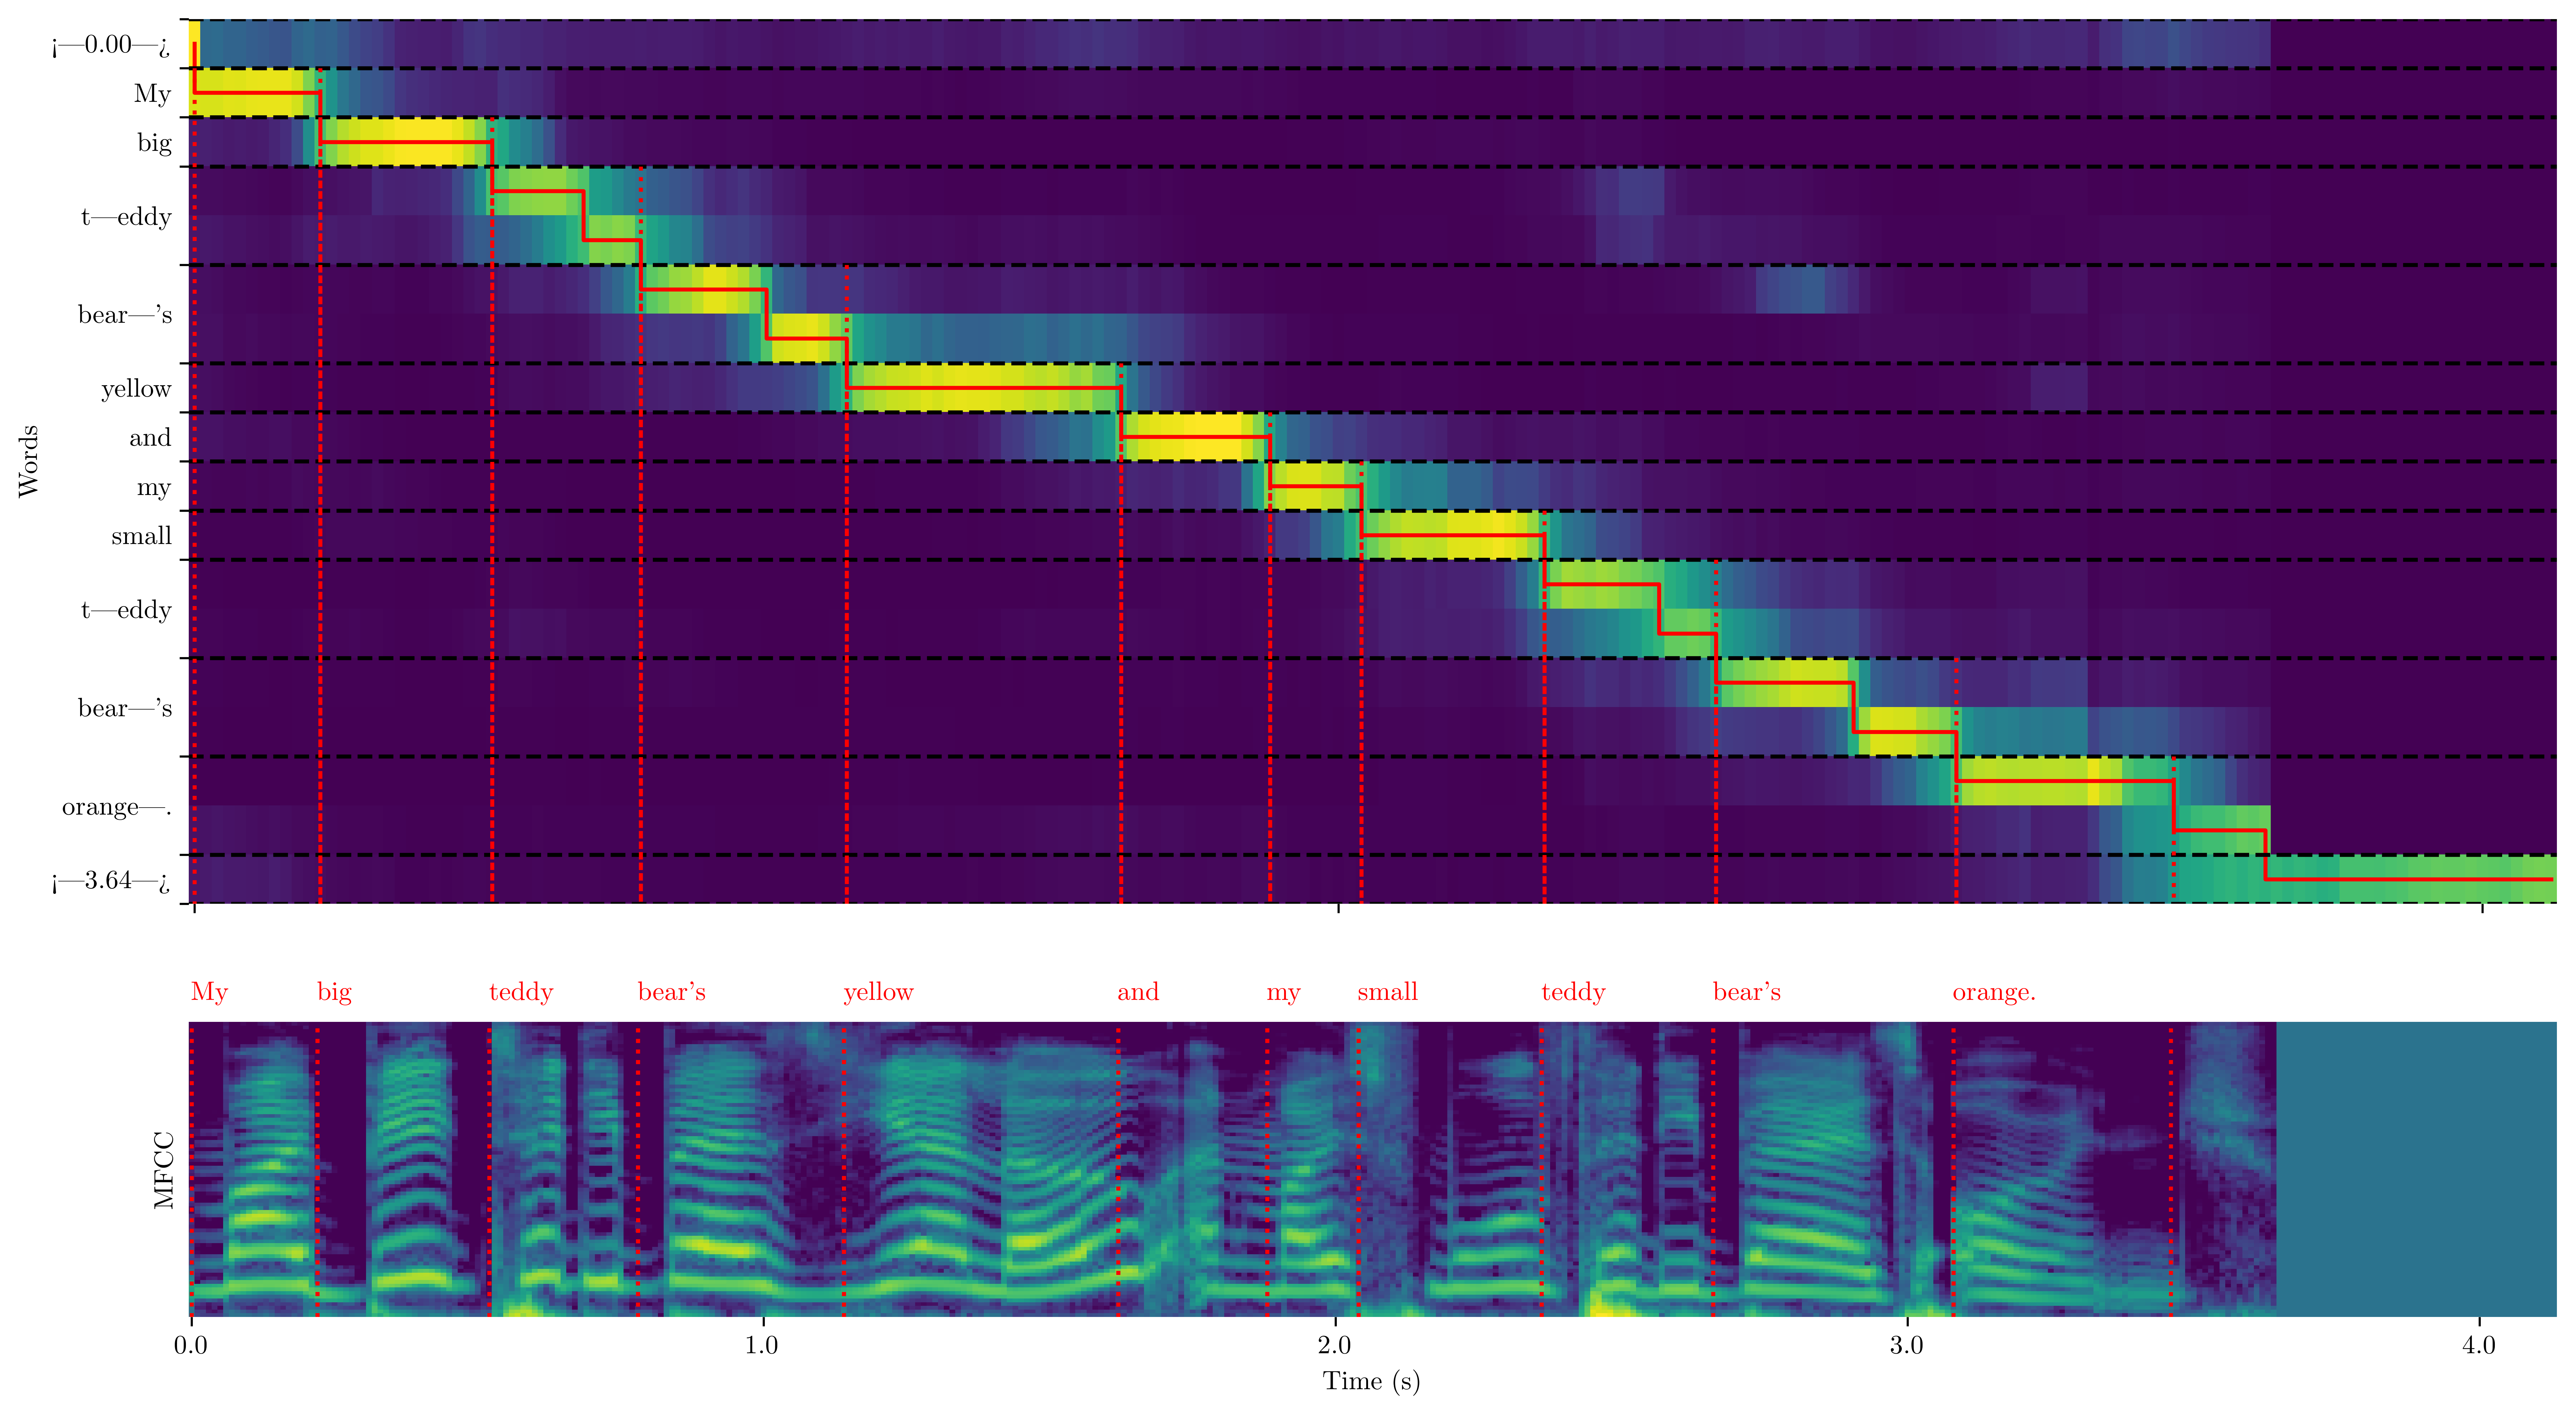
\includegraphics[width=\textwidth]{images/mfcc-with-words.png}
  \caption{Word alignments example}
  \label{fig:word-alignments-example}
\end{figure}

Figure \ref{fig:word-alignments-example} was generated using the \emph{whisper-timestamped} library\cite{whisper-timestamped, whisper-ts-dtw-paper, whisper}.
The top plot shows \say{the transformation of cross-attention weights used for the [word] alignment}\cite{whisper-timestamped}.
Notice that the words 'teddy' and 'bears' are split into subwords.

The aforementioned \emph{whisper-timestamped} library is able to assign confidence scores to each word, computed as the exponential of the mean of the $\log$ probabilities of each subword token in a given word.
Though based on probability scores which may not be wholly representative of confidence (as discussed in section \ref{sec:litreview-confidence}), operating on individual words rather than whole utterances should provide more detail of the per-word scores than \texttt{avg\_logprob} does.

\section{A System For Transcription}
\mycomment{
  I reckon this section shouldn't use screenshots yet, just give examples of coloured text, ordering and blanking.
  Save screenshots for Implementation chapter
}

\chapter{Implementation}\label{ch:implementation-and-testing}

The aim of this chapter is to provide some more insight into the choices made while implementing the design as discussed in the previous chapter and explain the motivations that lead to those choices.

\section{Data Processing}

TextGrid data was broken into 'utterances' using a script called \texttt{get\_utterances} (available in appendix \ref{appendix:get-utterances}).
This script takes as input a directory containing TextGrid data, an output directory and threshold values for the minimum break length and maximum pause length allowed in an utterance.
The output is in JSON format, generating a file to which other data is added.

The second step is to use the script \texttt{segment\_audio} to split up audio files into individual utterances within directories given the title of the orginal conversation they were extracted from.
This code is available in appendix \ref{appendix:segment-audio}.
Upon completion, the ouput of this script is a directory with subdirectories containing hundereds of audio files.

Thirdly, the script \texttt{do\_whisper\_confidence} was run (available in appendix \ref{appendix:do-whisper}) using the University of Sheffield's Bessemer HPC cluster\cite{shef-hpc}.
GPU clusters on Bessemer have access to Nvidia V100 GPUs with 32GB of VRAM, enabling transcriptions to be generated with Whisper very quickly.
Instead of using the standard Whisper model, the \emph{whisper-timestamped}\cite{whisper-timestamped} library is used because it can calculate word-level confidence scores.

The fourth and fifth steps to process data were to run the scripts \texttt{normalise\_text} and \texttt{calculate\_wer} (available in appendices \ref{appendix:normalise-text} \& \ref{appendix:calculate-wer} respectively).
The first of these scripts runs a text normaliser which is packaged with Whisper\cite{whisper} to perform English text normalisation, then the second script calculates WER scores and finds the per-word confidence scores for each word in the ouput.
WER is calculated using the \emph{jiwer}\cite{jiwer} library.

\begin{figure}[p]
\centering
\begin{BVerbatim}
"0": {
  "start": 15.04,
  "end": 15.74,
  "transcript": "okay",
  "whisper": {
    "text": "okay",
    "segments": [
      {
        "id": 0,
        "seek": 0,
        "start": 0.0,
        "end": 0.4,
        "text": " OK.",
        "tokens": [
          50363,
          7477,
          13,
          50440
        ],
        "temperature": 0.0,
        "avg_logprob": -0.7832436561584473,
        "compression_ratio": 0.2727272727272727,
        "no_speech_prob": 0.02687731385231018,
        "confidence": 0.317,
        "words": [
          {
            "text": "OK.",
            "start": 0.0,
            "end": 0.4,
            "confidence": 0.317
          }
        ]
      }
    ],
    "language": "en"
  },
  "confidence_scoring": {
    "words": "okay",
    "confidence_scores": [
      0.317
    ],
    "utterance_confidence": 0.317
  },
  "wer": 0.0,
  "avg_logprob": -0.7832436561584473,
  "file_measures": {
    "wer": 0.11153358681875793
  }
},
\end{BVerbatim}
  \caption{Example JSON entry from output}
  \label{fig:json-output-example}
\end{figure}

\clearpage
An example entry from the JSON output is presented in figure \ref{fig:json-output-example}.
The decision was made to preserve all of the output data from Whisper, meaning each entry is quite long.
An entry can be identified based on its filename and the number which indexes the entry ("0" in this case), where the filename of the accompanying audio segment has the same identifier (\texttt{000.wav} in this case).
As this example is the first entry in an output file, it contains a field called \texttt{file\_measures} which tracks the overall WER for the entire file.

This does, however, lead to the issue of readability re-emerging.
One of the goals of switching to JSON from TextGrid format was to improve the readability of the raw data.
Despite being kept in neat utterances, the data is not easily read as it is largely metadata rather than just the text.
Changing this would require removing some of the metadata (e.g. removing this 'words' field from the 'whisper' field), though the need for data preservation was ultimately considered paramount and thus the data remained in this format.

\subsection{Audio Issue}

During the first few experiments processing data through the script pipeline it was discovered that some audio files were being transcribed very poorly.
It was assumed that the same channels were labeled 'A' and 'B' for all of the recordings, however around half of the recordings use the opposite channel to the other.
This is important because the reference transcript TextGrid files are all labeled 'A' and 'B', thus the wrong audio channel had been segmented.

This issue was quickly diagnosed by calculating file-averages of the \texttt{no\_speech\_prob} output by Whisper, where it was discovered that half of the recordings were mostly silent (i.e. the speaker was listening to the other and not talking).
The conversations that had used the wrong channel were all discovered and the audio was re-segmented using the other channel.
The final corpus used for evaluation did not contain any of these errors.

\section{Demo Software}

The demo software's front-end is built using \emph{Textual}\cite{textual}, a Python libary for terminal-based graphical applications.
A terminal-based system was decided on to ensure compatibility across operating systems while using Python, as other techniques like \emph{PyQt}\cite{pyqt} do not display the same on all OSs.
Rich comes with various 'widgets' which enable quick and simple building of terminal applications, including the \texttt{DataTable} which was used for the demo software.
The code for the frontend is available in appendix \ref{appendix:asr-app}.

To gather results, highlight and blank text, play audio and order results, a backend was developed consisting of a simple class for each row and a class to represent all of the data in the table.
The backend code is available in appendix \ref{appendix:audio-data-link}.

\subsection{Caveats}

The demo software lacks the ability to be used as a real piece of computer-aided transcription software;
it can't take user input and has occasional audio glitches.

These problems prevent it from being used in any setting outside of simple demonstration and would require modification to both the front-end design and the method for playing audio.
Audio glitches are relatively uncommon and dissipate once the user plays a piece of audio multiple times, though if the system is intended to be used accurately the audio should be reliable and incapable of confusing a listener.
User input could be taken by, for example, adding a new column which takes keyboard input or allowing users to overwrite 'blanked out' sections of text.


\bibliographystyle{acm} 
\bibliography{analysis}

\begin{appendices}
\chapter{An Appendix of Some Kind}

Lorem ipsum dolor sit amet, consectetuer adipiscing elit. Aenean commodo ligula eget dolor. Aenean massa. Cum sociis natoque penatibus et magnis dis parturient montes, nascetur ridiculus mus. Donec quam felis, ultricies nec, pellentesque eu, pretium quis, sem. Nulla consequat massa quis enim. Donec pede justo, fringilla vel, aliquet nec, vulputate eget, arcu. In enim justo, rhoncus ut, imperdiet a, venenatis vitae, justo. Nullam dictum felis eu pede mollis pretium. Integer tincidunt. Cras dapibus. Vivamus elementum semper nisi. Aenean vulputate eleifend tellus. Aenean leo ligula, porttitor eu, consequat vitae, eleifend ac, enim. Aliquam lorem ante, dapibus in, viverra quis, feugiat a, tellus. Phasellus viverra nulla ut metus varius laoreet. Quisque rutrum. Aenean imperdiet. Etiam ultricies nisi vel augue. Curabitur ullamcorper ultricies nisi. Nam eget dui. Etiam rhoncus. Maecenas tempus, tellus eget condimentum rhoncus, sem quam semper libero, sit amet adipiscing sem neque sed ipsum. Nam quam nunc, blandit vel, luctus pulvinar, hendrerit id, lorem. Maecenas nec odio et ante tincidunt tempus. Donec vitae sapien ut libero venenatis faucibus. Nullam quis ante. Etiam sit amet orci eget eros faucibus tincidunt. Duis leo. Sed fringilla mauris sit amet nibh. Donec sodales sagittis magna. Sed consequat, leo eget bibendum sodales, augue velit cursus nunc.

\chapter{Another Appendix}

Lorem ipsum dolor sit amet, consectetuer adipiscing elit. Aenean commodo ligula eget dolor. Aenean massa. Cum sociis natoque penatibus et magnis dis parturient montes, nascetur ridiculus mus. Donec quam felis, ultricies nec, pellentesque eu, pretium quis, sem. Nulla consequat massa quis enim. Donec pede justo, fringilla vel, aliquet nec, vulputate eget, arcu. In enim justo, rhoncus ut, imperdiet a, venenatis vitae, justo. Nullam dictum felis eu pede mollis pretium. Integer tincidunt. Cras dapibus. Vivamus elementum semper nisi. Aenean vulputate eleifend tellus. Aenean leo ligula, porttitor eu, consequat vitae, eleifend ac, enim. Aliquam lorem ante, dapibus in, viverra quis, feugiat a, tellus. Phasellus viverra nulla ut metus varius laoreet. Quisque rutrum. Aenean imperdiet. Etiam ultricies nisi vel augue. Curabitur ullamcorper ultricies nisi. Nam eget dui. Etiam rhoncus. Maecenas tempus, tellus eget condimentum rhoncus, sem quam semper libero, sit amet adipiscing sem neque sed ipsum. Nam quam nunc, blandit vel, luctus pulvinar, hendrerit id, lorem. Maecenas nec odio et ante tincidunt tempus. Donec vitae sapien ut libero venenatis faucibus. Nullam quis ante. Etiam sit amet orci eget eros faucibus tincidunt. Duis leo. Sed fringilla mauris sit amet nibh. Donec sodales sagittis magna. Sed consequat, leo eget bibendum sodales, augue velit cursus nunc.

\end{appendices}

\end{document}
